\documentclass[]{report}
\usepackage{amsmath}
\usepackage{amsfonts}
\usepackage{physics}
\usepackage{graphicx}
\usepackage{hyperref}
\usepackage{fullpage}
\usepackage{pythontex}
% Title Page
\title{Symmetry Group Equivariant Neural Networks for Physical Systems}
\author{Alexander J. Heilman}


\begin{document}
\maketitle

\begin{abstract} 
a
\end{abstract}

\tableofcontents

\chapter{Introduction: Machine Learning Applied to Materials Science}
The fundamental assumption in any mathematical model of a physical system is that some initial set of properties describing the state of a system fully determines it's future state. 

Physics is essentially the pursuit of rigorous mathematical models that accurately describe physical phenomena. Often these models of physics have some rationale behind them from which they are derived, but such models must always describe the data collected empirically.

Machine Learning (ML) describes a set of techniques which also assume there exists a map between some input space and some target property (though, perhaps, in an extremely complex manner). However, ML approaches generally start with some randomly-chosen but tunable model which is then iteratively tuned or 'trained' to better fit the data directly.
\[
\lbrace \nu_i\rbrace \rightarrow t
\]


\section{Graph Neural Networks}
Neural networks are a class of universal function approximators, composed layer-wise by functions $\mathcal{L}^1\circ\mathcal{L}^2\circ ... \circ \mathcal{L}^n $, where each layer-to-layer transition map $\mathcal{L}^i$ is a trainable function from some feature space associated with layer $L$ to a feature space associated with layer $L+1$.

Many modern approaches use a specific type of neural network, referred to as a Graph Neural Network (GNN), which act on data encoded in features associated with some representative graph (i.e. a collection of nodes and connections between them).
	
\chapter{Mathematical Background: Vector Spaces, Groups, and Hamiltonians}
At a high-level, the intent of this chapter is to introduce basic concepts of mathematical and apply these, almost as they're introduced, to problems related to physical systems. These concepts are fundamental to the definition and implementation of equivariant networks to these same problems.

\section{Preliminaries}

A group $G$ is a set with a binary, associative product defined between it's elements under which it is closed, and for which every element, there exists an inverse element (and which also contains an identity element).

A vector space is a combined set of vectors $\lbrace \hat{x}_i\rbrace$, equipped with an associate, commutative, and invertible binary operation $+$ between them,  and scalars $\lambda$, which form a field, with an additional operation of \textit{scalar multiplication} between scalars and vectors that is distributive an asssociative, with identities and inversions further inherited from the scalar field.

A bra-ket space is a pair of vector space (typically over $\mathbb{C}^n$) equipped with an additional inner product between vectors of a bra space $\langle \psi\vert$ and vectors of a  ket space $\vert \psi\rangle$, notated as $\langle \psi\vert \psi\rangle$. These two vector spaces are related by the complex transposition operator, denoted by $^{\dagger}$, as:
\begin{align*}
\vert \psi\rangle^{\dagger}&=\langle \psi\vert \\
(\langle \psi\vert )_{i}&=(\vert \psi \rangle )_{i}^*
\end{align*}
We often care further about sets of operators $\hat{T}$ acting on bra-ket spaces, typically groups of operators that form a (reducible) representation of some abstract group.


\section{Hamiltonian Group}
Consider a physical system that obeys some particular Hamiltonian $H$ with eigenfunctions $\psi^{(i)}(\vec{r})$ and eigenvalues $E^{(i)}$.
$$
H\psi^{(i)}(\vec{r})=E^{(i)}\psi^{(i)}(\vec{r})
$$
Now, we define the group of this Hamiltionian $\mathcal{H}$ to be the group of all operations $h_j \in \mathcal{H}$ with representations (generally reducible) $\mathcal{O}(h_j)$ that leave $H$ invariant when acting on it's input space $\vec{r}$ so that:
$$
H(\mathcal{O}(h_j)\vec{r}) = H(\vec{r})
$$
In this case, the group representations $\mathcal{O}$ acting on the input space $\vec{r}$ can be seen to commute with $H$, in which case they must have simultaneous eigenfunctions $\psi(\vec{r})$.
$$
[H,O]=0 \quad \Rightarrow \quad \mathcal{O}(h_j)H\psi^{(i)}(\vec{r}) = E_i\psi^{(i)}(\vec{r})
$$ 

\subsection{Example: $D_2$ Oscillator Hamiltonian}
Consider the Hamiltonian of a pair of atoms separated by a distance of $d$.
This is a physical system with $D_2$ symmetry. 

\subsection{Example: Tight-Binding Hamiltonian}


\section{Representations of Groups}
A group representation $\rho:G\rightarrow GL(V)$ is a map from a set of group elements $G$ to a set of elements in the general linear group $GL(V)$ over a vector space $V$, which preserves group multiplication in cases of composition in $GL(V)$. In general, maps that preserve the action of the group in the codomain are referred to as homomorphisms.

A faithful representation is one which acts as a bijection, that is, each group element gets mapped to a unique element in the representation space. Every group has at least one representation, the trivial representation, which maps every group element to the number 1, so that the group multiplication is trivially preserved; however, the trivial representation is clearly not faithful. Finite order groups always admit at least one faithful representation, the regular representation, which maps each element to a corresponding permutation matrix. However, this representation space (of size $N\times N$, where $N$ is the order of the group) is rather large. Often, groups admit smaller representations, which leads to considerations of whether there exist `atomic' or smallest representation, which are referred to as irreducible representations.


\subsection{Irreducible Representations}
Irreducible representations essentially act as the building blocks of all possible representations of a group. In general, a representation $\rho$ is decomposable as a direct sum of irreducible representations $\Gamma^{(\alpha)}$ as:
\begin{equation}
\rho = \bigoplus_{\alpha}c_{\alpha}\Gamma^{(\alpha)}
\end{equation}
where $\alpha$ indexes the irreducible representations of the group and the expansion coefficient $c_{\alpha}$ is some positive integer. The coefficient of this expansion is derivable from the characters of $\rho$ and $\Gamma^{(\alpha)}$ as:
\begin{equation}
c_{\alpha}=\frac{1}{N}\sum_{g\in G}\big[\chi^{(\alpha)}(g)\big]^*\chi(g)
\end{equation}
The number of irreducible representations $n_{\Gamma}$ of a group is equal to the number of equivalence classes of a group $n_c$.
\begin{equation}
n_{\Gamma}=n_c
\end{equation}
Furthermore, the sum of the squares of the dimensions of the irreducible representations $d_{\alpha}$ is equal to the number of group elements $N$ as:
\begin{equation}
	N = \sum_{\alpha}d_{\alpha}^2
\end{equation}


\subsection{Physically Irreducible Representations}
Often in applications to the physical sciences, we wish to have a set of atomic real representations which are often termed \textit{Physically Irreducible Representations}. These may be constructed by taking the direct sum of a complex irrep and it's conjugate irrep (with a further change of basis if neccessary).

\subsection{Characters}
The explicit form of a representation is, in general, dependent upon a particular choice of basis and thus hard to characterize universally. The trace of a matrix, however, is invariant under change of basis. This motivates the definition of the character $\chi^{\alpha}(g)$ of a representation $\Gamma^{(\alpha)}$ for group element $g$, defined as:
\begin{equation}
	\chi^{\alpha}(g)=\text{Tr}\Big[\Gamma^{(\alpha)}(g)\Big]
\end{equation}
The characters are basis-independent by construction and allow one to universally characterize the representations of a group.
	
\subsection{Schur-Weyl Indicator}
The nature of a given representation may be given by the Schur-Weyl Invariant or Indicator, defined as:
$$
\frac{1}{\vert G\vert}\sum_{g\in G}\chi(g^2)=\begin{cases}
	-1 & \text{Symplectic}\\
	\ 0 & \text{Complex} \\
	\	1& \text{Real} \\
\end{cases}
$$
	
	
\section{Basis Functions}
The general linear group $GL(V):V\rightarrow V$ is the set of linear operators acting on the vector space $V$. Group representations map elements $g\in G$ to elements $M\in GL(V)$, which have a natural action on the underlying vector space $V$.

All vector spaces $V$ necessarily have sets of basis functions $\lbrace \psi_i\rbrace $ that span their space. Under some set of symmetry operations $G$ with a representation $O_G$ acting on a vector space, the basis functions may be labeled by the irreducible representations $\lbrace\gamma_{ i}\rbrace$ as s $\lbrace \psi_{\gamma i}\rbrace $ which span 

\subsection{SO(3) Basis Functions \& Wigner $\mathcal{D}$ Matrices}
Spherical harmonics $Y_{\ell}^m$ are a set of functions that form a basis for functions on the surface of a sphere, analogous to the sinusoidal functions correspondence to a plane. 
$$
f(\theta,\phi)=\sum_{\ell, m}f_{\ell}^mY_{\ell}^m(\theta,\phi)
$$
The $2\ell+1$ dimensional invariant subspaces $V_{\ell}$ transform according to the \textit{Wigner $\mathcal{D}$-matrices} as:
$$
\mathcal{D}^{\ell}(R)Y_{\ell}^m(\theta,\phi)=\sum_{m}\mathcal{D}_{mm'}^{\ell}(R)Y_{\ell}^{m'}
$$

\subsubsection{Explicit Form of Wigner-$\mathcal{D}$ Matrices}
The $\mathcal{D}$ matrices are often parameterized by Euler angles $\theta,\phi,\Omega$, here chosen to be in the $z\rightarrow y\rightarrow z$ convention. Since rotations about the $z$-axis are chosen to behave particularly nice in the usual convention of $ Y^{\ell}_m$, we may assume such rotations are diagonal, i.e.:
$$
\mathcal{D}_z(\theta)_{m,m'}\equiv \mathcal{D}(\theta, 0, 0) _{m,m'} = \mathcal{D}(0,0,\theta) _{m,m'} = e^{-im\theta}\delta_{m,m'}
$$
The non-trivial consideration then is that of it's form for rotations about the $y$-axis. Rotations about the non-trivial Euler angle axis are usually defined as the Wigner little-$d$ matrix:
$$
d(\phi)_{m,m'}\equiv \mathcal{D}(0,\phi, 0) _{m,m'}
$$

\subsection{Irreducible Representations of Permutation Groups}
The irreducible representations of the permutation (or symmetric) groups $S_n$ may be represented and cataloged diagrammatically with a set of objects known as Young Diagrams. From these diagrams, we may further construct symmetrizers which act as projection operators for relevant basis sets. 

\subsubsection{Young Diagrams}
Young diagrams of order $n$ are left-justified arrangements of boxes into $k$ rows stacked vertically in non-increasing order. 
\begin{figure}\centering
	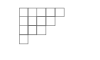
\includegraphics[scale=0.6]{youngdiagram-ex.pdf}
	\caption{Example Young diagram of shape $(5,4,3,1)$.}
\end{figure}
A Young diagram is said to be of some shape $\lambda:(\lambda_1,\lambda_2,...,\lambda_k)$, where $\lambda_i$ refers to the depth of row $i$ and $\lambda_{i+1}\leq\lambda_i\leq\lambda_{i-1}$. 

We can then form a set of Young tableaux from diagrams by filling in the boxes from a set of ordered indices $\lbrace x_1,x_2,...,x_k\rbrace$ corresponding to tensor components $T^{x_1x_2...x_k}$.  A standard tableu is one filled with indices $x_i$ (without repeats) with entries increasing in index $i$ down each column and across (to the right) rows.
\begin{figure}\centering
	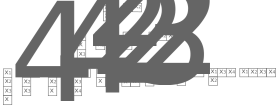
\includegraphics[scale=0.42]{youngtableaux-ex.pdf}
	\caption{Standard Young tableaux for diagrams of at most 4 boxes.}
\end{figure}

Each of these standard tableaux correspond to an invariant subspace under $S_k$. From these tableau, we may construct so-called \textit{Young Symmetrizers}, which project tensors onto their corresponding $S_k$-invariant subspace. 

A Young symmetrizer $P_{\lambda}$ corresponding to tableau $\lambda$ is composed of a compound set of symmetrizing operations $s_{\lambda}$ and antisymmetrizing operations $a_{\lambda}$, scaled by an overall normalization constant $C_{\lambda}$:
$$
P_{\lambda} = \mathcal{C}_{\lambda}s_{\lambda}a_{\lambda}
$$
Where here, we adopt the convention of anti-symmetrization before symmetrization, following that in Itin \cite{Itin-r3}.

The symmetrizing operator $s_{\lambda}$ for a diagram $\lambda$ is composed of a product of symmetrizers $\mathcal{S}(\mathcal{I})$, where $\mathcal{I}$ ranges over all subsets of indices corresponding to some vertically stacked set of indices in tableau $\lambda$, i.e.:
$$
s_{\lambda} = \prod_{\mathcal{I}\in \text{Cols}(\lambda)}\mathcal{S}(\mathcal{I})
$$
where $\text{Cols}(\lambda)$ represents the set of disjoint subsets of indices down each column, and symmetrizers $\mathcal{S}$ are defined to act on tensors $T$ component-wise as:
$$
\big[\mathcal{S}(\mathcal{I})T\big]_{ijk...}= \sum_{\sigma_{\mathcal{I}}}T_{\sigma_{\mathcal{I}}(ijk...)}
$$
where $\sigma_{\mathcal{I}}$ are permutations of index subset $\mathcal{I}$.

Similarly, the antisymmetrizing operator $a_{\lambda}$ can be constructed as a product of antisymmetrizers:
$$
a_{\lambda} = \prod_{\mathcal{I}\in \text{Rows}(\lambda)}\mathcal{A}(\mathcal{I})
$$
where $\text{Rows}(\lambda)$ represents the set of  disjoint subsets of indices across each entire row, and antisymmetrizers $\mathcal{A}$ are defined as:
$$
\big[\mathcal{A}(\mathcal{I})T\big]_{ijk...}= \sum_{\sigma_{\mathcal{I}}}\text{sgn}(\sigma_{\mathcal{I}})T_{\sigma_{\mathcal{I}}(ijk...)}
$$
where, again, $\sigma_{\mathcal{I}}$ range over all permutations of index subset $\mathcal{I}$.



The normalization constant $C_{\lambda}$ may be derived from the shape of the underlying Young diagram according to the \textit{hook-length formula}, given below, where $\text{hook}(\alpha,\beta)$ returns the number of boxes crossed by a hook coming up (from below) column $\beta$ and out of the diagram to the right in row $\alpha$.
$$
C_{\lambda}= \prod_{(\alpha,\beta)\in \lambda}\frac{1}{\text{hook}(\alpha,\beta)}
$$
Furthermore, the number of independent components $N_{\lambda}$ of a tensor subspace corresponding to some Young tableau with shape $\lambda$ may also be derived from the diagram by a related hook-length formula:
$$
N_{\lambda}= \prod_{(\alpha,\beta)\in \lambda}\frac{n-\alpha+\beta}{\text{hook}(\alpha,\beta)}
$$
where $n$ is the dimension of the vector space forming the tensor space. 

Thus, the standard Young tableaux of $k$ boxes can be used to decompose an arbitrary tensor space into a set of $GL$ invariant subspaces with known symmetries (under permutation of indices) by way of corresponding Young symmetrizers. These known symmetries will be relevant in the further decomposition of these subspaces by way of contractions with the metric tensor, and the fully antisymmetric tensor, discussed below.
\begin{figure}\centering
	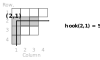
\includegraphics[scale=0.6]{hook-ex.pdf}
	\caption{Example value of $\text{hook}(2,1)$ for a diagram of shape $\lambda:(4,3,3,1)$. Note that it's corresponding normalization constant is $C_{\lambda}=1/33600$.}
\end{figure}

\subsubsection{Schur-Weyl Duality}

Under the joint action of the symmetric group $S_k$ and $GL_n$ acting on a tensor of rank-$k$ over $(\mathbb{C}^n)^{\otimes k}$, the tensor space may be decomposed into a direct sum of tensor products of representations of $S_k$, $\pi_k$ and representations of $GL_n$, here $\rho_n$, simultaneously indexed by the set of Young diagrams $\lambda$ of order $k$. That is,
$$
\underbrace{\mathbb{C}^n\otimes ... \otimes\mathbb{C}^n}_k= \bigoplus_{\lambda}\pi^{(\lambda)}_{k}\otimes\rho_n^{(\lambda)}.
$$
This is a statement of the Schur-Weyl duality without proof. The point here though is that the representations under $GL$ of a complex tensor product space, are indexed by the same set (that is, they both are described by the same underlying structure) as the representations under $S$.  Thus, we consider the $GL$ decomposition to be synonymous here with the symmetric group $S$ decomposition.

\subsection{Irreducible Representations of $\mathbb{R}^3$ Point Groups}
A point group is defined as a group that preserves the position of (at least) a chosen origin point in some space, typically $\mathbb{R}^2$ or $\mathbb{R}^3$. In $\mathbb{R}^3$, they're typically classified into symmetric groups $S_n$; cyclic groups $C_n, C_{nh},C_{nv}$; dihedral groups $D_{n},D_{nh}, D_{nd}$; tetrahedral groups $T_n,T_{nd}$; octahedral groups $O_n,O_{nd},O_{nh}$; and icosahedral groups $I_n,I_{nd}$.

These groups all admit a simultaneous representation on $\mathbb{R}^3$ defined sometimes as \textit{Jones' faithful representation}. Their irreducible representations $\Gamma^{(\alpha)}$ are of dimension $d_{\alpha}\leq 3$.

\subsubsection{Crystallographic Restrictions}
Only certain point groups are compatible with crystallographic translational symmetry. These are referred to as the\textit{ crystallographic point groups}.

\subsection{Irreducible Representations of Translational Groups}
A translational group $T$ in some space is one which allows for a shifting of the origin of a vector space generated by some set of non-co-linear vectors ${\vec{r}_{i}}$ in the space. Translational groups in arbitrary dimension are Abelian.

\subsubsection{Empty Space \& Plane Waves}
Since translational groups are Abelian, their irreps are necessarily all one-dimensional. In the plane wave basis, we essentially reduce Cartesian components into these one-dimensional invariant subspaces with indexes $\vec{k}$ which determine their transformation under some translation $T_{\vec{r}}$  along one axis $\vec{r}$ by:
$$\psi_{\vec{k}} \xrightarrow{T_{\vec{r}}} T_{\vec{r}}\psi_{\vec{k}}=e^{-i\vec{k}\cdot\vec{r}}\psi_{\vec{k}}$$
This corresponds exactly to the a Fourier transform of arbitrary functions.
 
 
\subsubsection{Bravais Lattices \& Bloch Functions}
Only a finite number of distinct crystallographic translational symmetries may be represented in $\mathbb{R}^n$. These are referred to as Bravais lattices; in $\mathbb{R}^2$ there are 7, and in $\mathbb{R}^3$ there are 14.
These consist of translation along $n$ non-co-linear axis $\lbrace \vec{a}_i \rbrace$ in $n$-dimensional space.

For scalar valued functions $f(\vec{r})$ on $\mathbb{R}^n$, the basis functions $u_{x_1,x_2, ... x_n}$ labeled under these groups transform independently along projections onto each of these axis with multiples $x_1, x_2,...x_n$, transforming as:
$$u_{a_1,a_2, ... a_n} \xrightarrow{T_{b_1,b_2, ... b_n}} T_{b_1,b_2, ... b_n}u_{a_1,a_2, ... a_n}=e^{-2\pi i(a_1b_1+a_2b_2+ ... a_nb_n)}u_{a_1,a_2, ... a_n}$$
In quantum mechanics where $f$ is taken to be wave function, these basis functions are commonly referred to as the \textit{Bloch functions} of a given crystal system.% though a further phase may be allowed in these cases due to additional symmetries of quantum systems.

\section{Projection Operators}
For an arbitrary vector space $V$ with some (possibly reducible) representation $\hat{O}(G)$ of group $G$ that acts on it, a set of projection operators $\hat{P}^{\mu}_{ij}$ may be constructed for subspaces $V_{\mu}$, which each transform as some irreducible representation $\Gamma^{\mu}$ of $G$ (spanned by basis functions $\psi^{\mu}_i$). The most extensive set of these projection operators is defined as follows:
$$
\hat{P}^{\mu}_{ij} = \frac{d_{\mu}}{N_G}\sum_{g\in G}\mathcal{D}^{\mu \dagger}(g)_{ij}\hat{O}(g) \quad\quad \Big(=\vert\psi_{i}^{\mu}\rangle\langle\psi_{j}^{\mu}\vert \Big)
$$
\begin{center}
Where we then further define the projection onto an arbitrary basis function: %$\vert\psi^{\mu}_i\rangle$:
$$\hat{P}^{\mu}_{i}\equiv \hat{P}^{\mu}_{ii}$$
and then the projection onto the total subspace $V_{\mu}$:
$$
\hat{P}^{\mu}\equiv \sum_{i}\hat{P}^{\mu}_{ii} =  \frac{d_{\mu}}{N_G}\sum_{g\in G}\chi^{\mu *}(g)\hat{O}(g)
$$
\end{center}
Note that the definition of the projection operators $\hat{P}^{\mu}_{ij}$ and $\hat{P}^{\mu}_{i}$ require explicit definitions of each of the irreducible representations $\mathcal{D}^{\mu}$ (i.e., some basis must be chosen); $\hat{P}^{\mu}$ however may be implemented from only the character table.

\section{Subgroup Chains}
Often, large symmetry groups contain non-trivial subgroups, which themselves may contain further non-trivial subgroups. These relations are conveyed by subgroup chains written for instance, as:
$$
O(3)\supset O(2) \supset C_i
$$
where we declare $O(3)$ contains $O(2)$ which further contains $C_i$. The relevance of these non-trivial subgroup chains is that these structures make clear that we may assume some coordinate system in which basis functions are labeled simultaneously by the irreps of each symmetry group in the chain.

For example, the parity-dependent spherical harmonics $(Y_{\ell}^m)^{p}$ are defined in terms of three indices $\ell, m, p$ where $\ell$ is a label inherited from it's $O(3)$ symmetry, $m$ from $O(2)$, and $p$ from $C_i$. Under the full group of 3D rotations, the invariant subspaces of $\mathbb{R}^3$ may only be labeled by rotational order $\ell$ with $2\ell+1$ (degenerate) basis functions. It's only by choosing a convenient coordinate system for when only z-axis rotations are considered (i.e. rotations about an arbitrarily chosen axis) do we resolve the basis functions further by their newly inherited label $m$. Parity values follow similarly from inversion under $C_i$.

\section{Products of Irreducible Subspaces}
Often in applications to physics involving group irrep indexed basis functions, we encounter tensors products $\otimes$ (equivalently for our discussion, direct products) of basis functions and their corresponding spaces they span. Coupling and Clebsch-Gordan coefficients describe simple decompositions of tensor products of such irrep-labeled basis functions. Wigner 3-$j$ and higher symbols describe similar scenarios with products of more basis functions simultaneously, though additional stipulations are made in their definitions so they inherit more symmetry. 

Noteably, applications of the coefficients and symbols defined below (as well as Dirac notation in general) often admit a diagrammatic description, which may facilitate high-level reductions of otherwise complicated products. 


\subsection{$SO(3)$: Clebsch-Gordan Coefficients}
The Clebsch-Gordan coefficients are elements of a matrix $C^{\ell_f  m_f}_{\ell_1  m_1\ell_2 m_2}$ that block-diagonalize the tensor product space of two spherical harmonic spaces.
$$
Y_{\ell_1}^{m_1}(\Omega)Y_{\ell_2}^{m_2}(\Omega)=\sum_{\ell_3, m_3}\sqrt{\frac{(2\ell_1+1)(2\ell_2+1)}{4\pi(2\ell_3+1)}}C^{\ell_3m_3}_{\ell_1m_1\ell_2m_2}C^{\ell_30}_{\ell_1 0\ell_2 0}Y_{\ell_3m_3}(\Omega)
$$
with unit-integral-normalization (with the leading radical omitted in the Racah semi-normalization).

\subsubsection{Wigner n-$j$ Symbols}
The C-G coefficients may be derived from the set of Wigner 3-$j$ symbols, which are defined such that their symmetries under permutation are greater, and thus their specific values may be more efficiently stored. Below, the most common set of Wigner coefficients are presented.

\subsubsection*{1-$jm$}
The 1-$jm$ symbol acts as a metric for spherical states.
$$ 
{\begin{pmatrix}j\\m\quad m'\end{pmatrix}}:={\sqrt {2j+1}}{\begin{pmatrix}j&0&j\\m&0&m'\end{pmatrix}}=(-1)^{j-m'}\delta _{m,-m'}
$$
\subsubsection*{2-$jm$}
The 2-$jm$ symbol describes the coupling of pairs of vectors to the trivial irrep space.
$$
\begin{pmatrix}
	j_1 & j_2  \\
	m_1 & m_2 
\end{pmatrix} = \sqrt{2j_1+1}\delta_{-j_1-m_1}^{j_2m_2}
$$
In this case, it's diagonal since the only way a product of two states transforms trivially is if they're related by complex conjugation (i.e. $j_2=-j_1$).

\subsubsection*{3-$jm$}
The Wigner 3-$j$ symbols are defined such that their sum over the tensor product of three $SO(3)$ subspaces is exactly the zero, i.e. the coefficients appearing in the relation:
$$
\sum_{m_1,m_2,m_3}\begin{pmatrix}
	j_1 & j_2 & j_3 \\
	m_1 & m_2 & m_3
\end{pmatrix}\vert j_1m_1\rangle\vert j_2m_2\rangle\vert j_3m_3\rangle = \vert 00\rangle
$$
They are related to the C-G coefficients as:
$$
\begin{pmatrix}
	j_1 & j_2 & j_3 \\
	m_1 & m_2 & m_3
\end{pmatrix} = \frac{(-1)^{j_1-j_2-m_3}}{\sqrt{2j_3+1}}c_{j_1m_1j_2m_2}^{j_3-m_3}
$$
They are defined explicitly as:
{\small
\begin{align*}{\begin{pmatrix}j_{1}&j_{2}&j_{3}\\m_{1}&m_{2}&m_{3}\end{pmatrix}}&\equiv \delta (m_{1}+m_{2}+m_{3},0)(-1)^{j_{1}-j_{2}-m_{3}}{}{\sqrt {\frac {(j_{1}+j_{2}-j_{3})!(j_{1}-j_{2}+j_{3})!(-j_{1}+j_{2}+j_{3})!}{(j_{1}+j_{2}+j_{3}+1)!}}}\ \times {}\\[6pt]&\times {\sqrt {(j_{1}-m_{1})!(j_{1}+m_{1})!(j_{2}-m_{2})!(j_{2}+m_{2})!(j_{3}-m_{3})!(j_{3}+m_{3})!}}\ \times {}\\[6pt]&\times \sum _{k=K}^{N}{\frac {(-1)^{k}}{k!(j_{1}+j_{2}-j_{3}-k)!(j_{1}-m_{1}-k)!(j_{2}+m_{2}-k)!(j_{3}-j_{2}+m_{1}+k)!(j_{3}-j_{1}-m_{2}+k)!}},\end{align*}}
\subsubsection*{6-$j$}

\begin{align*}{\begin{Bmatrix}j_{1}&j_{2}&j_{3}\\j_{4}&j_{5}&j_{6}\end{Bmatrix}}&=\sum _{m_{1},\dots ,m_{6}}(-1)^{\sum _{k=1}^{6}(j_{k}-m_{k})}{\begin{pmatrix}j_{1}&j_{2}&j_{3}\\-m_{1}&-m_{2}&-m_{3}\end{pmatrix}}\times \\&\times {\begin{pmatrix}j_{1}&j_{5}&j_{6}\\m_{1}&-m_{5}&m_{6}\end{pmatrix}}{\begin{pmatrix}j_{4}&j_{2}&j_{6}\\m_{4}&m_{2}&-m_{6}\end{pmatrix}}{\begin{pmatrix}j_{4}&j_{5}&j_{3}\\-m_{4}&m_{5}&m_{3}\end{pmatrix}}.\end{align*}

\subsubsection*{9-$j$}
$$
\begin{Bmatrix}j_{1}&j_{2}&j_{3}\\j_{4}&j_{5}&j_{6}\\j_{7}&j_{8}&j_{9}\end{Bmatrix}=\sum _{x}(-1)^{2x}(2x+1)\begin{Bmatrix}j_{1}&j_{4}&j_{7}\\j_{8}&j_{9}&x\end{Bmatrix}\begin{Bmatrix}j_{2}&j_{5}&j_{8}\\j_{4}&x&j_{6}\end{Bmatrix}\begin{Bmatrix}j_{3}&j_{6}&j_{9}\\x&j_{1}&j_{2}\end{Bmatrix}
$$

\subsection{Point Group Coupling Coefficients}
Coupling coefficients $U_{\alpha i,\beta j}^{\gamma n}$ are those  elements of the point groups analagous to Clebsch-Gordan coefficients of $SO(3)$, relating the direct sum decomposition space indexed by $\gamma$ to the tensor product spaces indexed by $\alpha,\beta$ as:
$$
\psi^{\gamma}_{n}=\sum_{ i, j}U_{\alpha i,\beta j}^{\gamma n}u^{\alpha}_iv^{\beta}_j
$$
 
These may be defined, from particular forms of representations $\Gamma^{\alpha},\Gamma^{\beta},\Gamma^{\gamma}$ for all point groups of interest from Dirl's formula \cite{dirl1979}:
$$
(U^{\gamma n}_{\alpha i \beta j})^m = \sqrt{\frac{d_{\gamma}}{N_{G}}}\Big(\sum_{g\in G}\Gamma^{\alpha}_{qq}(g)\Gamma^{\beta}_{ss}(g)\Gamma^{\gamma \dagger}_{aa}(g)\Big)^{-\frac{1}{2}}\cdot \sum_{g\in G}\Gamma^{\alpha}_{iq}(g)\Gamma^{\beta}_{js}(g)\Gamma^{\gamma\dagger}_{na}(g)
$$
It should be noted here that the definition of these coefficients thus requires explicit (fixed) forms for each irrep of each point group of interest.


\chapter{Equivariant Graph Neural Networks}




\section{Equivariance}
A function $f:X\rightarrow Y$ is equivariant with respect to a group $G$ if, for representations $\mathcal{D}_X$ and $\mathcal{D}_Y$ of $G$ (over spaces $X$ and $Y$, respectively), it satisfies:
$$
f(D_X(g)x) = D_Y(g)f(x) \quad\quad \forall g\in G
$$
Essentially, a function is equivariant with respect to some group if it 'commutes' with the representations of groups on it's input and output space. 

\subsubsection*{Invariance}
A special case of equivariance then is \textit{invariance}, where the representations of all group elements in the output space are identity (i.e. $D_Y$ is the trivial representation). That is, a function $f:X\rightarrow Y$ is invariant under a group $G$ if it satisfies:
$$
f\circ \mathcal{D}_X(g) = f \quad
\ \forall g\in G.
$$

\section{$SO(3)$ Equivariant Layers}
Since compositions of equivariant functions are themselves equivariant, we need only consider a set of basic equivariant functions which may then be composed layer-wise to construct arbitrarily large equivariant networks. Below, we give brief descriptions of four common equivariant functions %\cite{equivariant_cohen} 
used in such networks, namely: point-wise nonlinearities; self-interaction; pooling functions; and the heart of equivariant networks, equivariant convolution.

\subsection*{$SO(3)$-Equivariant Convolution}
Features and filters in $SO(3)$ networks are both associated with $SO(3)$ representations, or spherical harmonics.
Tensor products of these two representation spaces are equivariant under transformation of the two subspaces, i.e.:
$$
\mathcal{D}^V\otimes \mathcal{D}^W=\mathcal{D}^{V\otimes W}.
$$
By way of Clebsch-Gordan coefficients $c^{\ell_3m_3}_{\ell_1m_1\ell_2m_2}$, these tensor products of $SO(3)$ irreducible representations may be related to a third set of irreducible representations as \cite{sakurai}:
$$
(u\otimes v)_{\ell_o}^{m_o} = c_{\ell_1m_1\ell_2m_2}^{\ell_om_o}u_{\ell_1}^{m_1}v_{\ell_2}^{m_2}
$$
where $u$ and $v$ are harmonic vectors of order $\ell_1$ and $\ell_2$, respectively.
Since tensor products of representations are naturally equivariant, we may define $SO(3)$-equivariant convolution to be the scaled tensor product of the two representation spaces (i.e. that of the input feature space, and the filter space). Specifically, layer to layer convolutional maps $\mathcal{L}$ may be defined component-wise as\cite{tensorfieldnetworks}:
$$
\mathcal{L}^{\ell_o}_{acm_o}\big(\vec{r}_a,V_{acm_i}^{\ell_i}\big) = \sum_{m_f,m_i}c_{\ell_im_i\ell_fm_f}^{\ell_o m_o}\sum_{b}F^{\ell_f\ell_i}_{cm_f}(r_{ab})V_{bcm_i}^{\ell_i}
$$
where the filter function $F^{\ell_f\ell_i}_{cm_f}(r_{ab})$ depends only on the distance between point $a$ and $b$ (as opposed to directional dependence, to maintain equivariance). Instances of such functions then generally have independent, trainable parameters for different rotational orders $\ell_f, \ell_i$, azimuthal orders $m$, and channels $c$.
%To maintain equivariance, for an input feature set of the type described above,  through convolution with some filter $F$,  the filter also must be associated with a set of spherical harmonics, and thus also has an additional two indices $\ell_f$ and $m_f$. 

\subsection*{Self-Interaction}
Feature sets for individual objects may also update according to themselves as long as they act across $m$ for every $\ell$ and only update according to the different channels $c$. That is, functions of the form:
$$
V_{acm}^{\ell} \rightarrow  \sum _{c}W^{\ell}_{c'c}V_{acm}^{\ell}
$$
are also equivariant. Such functions we refer to as \textit{self-interaction} layers since they act node-wise such that no information is exchanged between nodes.

\subsection*{Non-Linearities}
We can also apply point-wise non linearities and maintain equivariance, as long as they only act on the $\ell=0$ (that is, the rotationally-invariant) features of each layer. Non-linearities applied to features with index $\ell>0$ break equivariance since rotations affect the values of specific components indexed by $m$.

\subsection*{Pooling}
Pooling, or aggregation, across all elements or objects (index $a$) while preserving the $m$ and $\ell$ indices is also equivariant. So functions of the form:
$$
M_{cm}^{\ell} = \text{AGG}_{a}(\lbrace V_{acm}^{\ell}\rbrace)
$$ 
where $\text{AGG}$ is an arbitrary aggregation function performed only over the object index $a$, are also available in the construction of $SO(3)$ networks. Typically, pooling layers are utilized in the final layer of models to generate global representations of material structures from node-wise, atomistic, representations.






\chapter{Crystal Group Equivariant Networks}

\medskip

\end{document}          
